\documentclass[12pt]{article}
\usepackage[utf8]{inputenc}
\usepackage[left=2.5cm, right=2.5cm, top=2.0cm]{geometry}
\usepackage{sectsty}
\usepackage{graphicx}
\usepackage{amsmath}
\usepackage{amssymb}
\usepackage{undertilde}
\usepackage{kbordermatrix}
\usepackage{listings}
\usepackage{ulem}
\usepackage{soul}
% \usepackage{tikz}
% \usepackage{pgfplots}
% \pgfplotsset{compat=1.16} 
\usepackage{siunitx}
\usepackage{pythonhighlight}
\usepackage{caption}
\usepackage{float}
\usepackage{url}
\usepackage{enumitem}
\usepackage{bm}
\usepackage{empheq}
\usepackage{tcolorbox}
\usepackage{framed}
\usepackage{xparse}
\usepackage{algorithm, algorithmic}
% \usepackage{algorithmic}
\usepackage{booktabs}
\usepackage{tabularx}
% ref packages
\usepackage{nameref}
% folowing  must be in this order
\usepackage{varioref}
\usepackage{hyperref}
\usepackage{cleveref}
\usepackage{mathtools}
\DeclareMathOperator*{\argmax}{arg\,max}
% \usepackage[shortlabels]{enumitem}
\tcbuselibrary{breakable}
\allowdisplaybreaks


%  ---------------------- COMMANDS ---------------------------
% Double underline
\def\dunderline#1{\underline{\underline{#1}}}

% Shorten nonumber command
\def\nnb{\nonumber}

% Shorten boldsymbol command
\def\bs#1{\boldsymbol{#1}}

% Algorithmic newline
\def\algonewline{\STATE{ }}

% Eigenvectors of
\def\eigvecof{\text{eigenvectors of }}

% Eigenvalues of 
\def\eigvalof{\text{eigenvalues of }}

% Enclose in square brackets
\newcommand{\enclb}[1]{\left[#1\right]}
% Enclose in parenthesis
\newcommand{\enclp}[1]{\left(#1\right)}
% Enclose in curly brackets
\newcommand{\enclc}[1]{\left\{#1\right\}}

% Annotate first argument, text in second argument
\newcommand{\overtext}[2]{\overbrace{#1}^{\mathclap{\text{#2}}}}
\newcommand{\undertext}[2]{\underbrace{#1}_{\mathclap{\text{#2}}}}

% Normalization constant in multivariate normal
\newcommand{\mvnconst}[1]{\frac{1}{(2\pi)^{d/2} |#1|^{1/2}}}

% Exponential factor in multivariate normal
\newcommand{\mvnexpo}[3][x]{\exp \left[  -{\frac{1}{2}} (#1 - #2)^T #3^{-1} (#1 - #2) \right]}

% Multivariate normal
\newcommand{\mvn}[3][x]{\mvnconst{#3} \mvnexpo[#1]{#2}{#3}}

% For numbering in align* environment
\newcommand{\numberthis}{\addtocounter{equation}{1}\tag{\theequation}}

%  Sum notation w/ limits as argument and index as option
\newcommand{\sumlim}[3][i]{\sum\limits_{#1=#2}^{#3}}

%  Product notation w/ limits as argument and index as option
\newcommand{\prodlim}[3][i]{\prod\limits_{#1=#2}^{#3}}

%  Sum notation with only information beneath
\newcommand{\sumnolim}[1]{\sum\limits_{#1}}

%  Integral notation w/ limits as argument and index as option
\newcommand{\intlim}[2]{\int\limits_{#1}^{#2}}

%  Integral over whole domain notation, no args
\newcommand{\intinf}{\int\limits_{-\infty}^{\infty}}

%  Partial derivative notation, arg1: numerator, arg2: denominator
\newcommand{\pfrac}[3][ ]{\frac{\partial^{#1} #2}{\partial #3^{#1}}}

%  Derivative notation, arg1: numerator, arg2: denominator
\newcommand{\dvfrac}[3][ ]{\frac{\text{d}^{#1} #2}{\text{d} #3^{#1}}}

% When doing Gauss-Jordan, create arrow showing operations
\newcommand{\ro}[1]{\xrightarrow{\mathmakebox[\rowidth]{#1}}}

% ----------------------INVIRONMENTS---------------------------
% Item list with title
\newenvironment{titlemize}[1]{%
  \paragraph{#1}
  \begin{itemize}}
  {\end{itemize}}

  % Enum list with title
\newenvironment{titleenum}[1]{%
  \paragraph{#1}
  \begin{enumerate}}
  {\end{enumerate}}

  % Augmented matrix (matrix with vertical line)
\newenvironment{sysmatrix}[1]
  {\left(\begin{array}{@{}#1@{}}}
  {\end{array}\right)}

 % Make matrices with more spacing
\makeatletter
\renewcommand*\env@matrix[1][\arraystretch]{%
  \edef\arraystretch{#1}%
  \hskip -\arraycolsep
  \let\@ifnextchar\new@ifnextchar
  \array{*\c@MaxMatrixCols c}}
\makeatother

% \renewcommand*{\arraystretch}{1.5}

\newlength{\rowidth}% row operation width
\AtBeginDocument{\setlength{\rowidth}{3em}}

\floatname{algorithm}{Algorithm}
\renewcommand{\algorithmicrequire}{\textbf{Input:}}
\renewcommand{\algorithmicensure}{\textbf{Output:}}

\begin{document}
\title{\textbf{INF367A Exercise 10}}
\author{Naphat Amundsen}
\maketitle
\sectionfont{\fontsize{14}{15}\selectfont}
\subsectionfont{\fontsize{12}{15}\selectfont}
\subsubsectionfont{\fontsize{12}{15}\selectfont}
\graphicspath{ {./images/} }

\ifx
\begin{figure}[H]
	\centering
	\includegraphics[scale=0.8]{Figure_2}
	\caption{Insert caption here}
\end{figure}
\fi
\ifx
\begin{figure}[H]
	\centering
	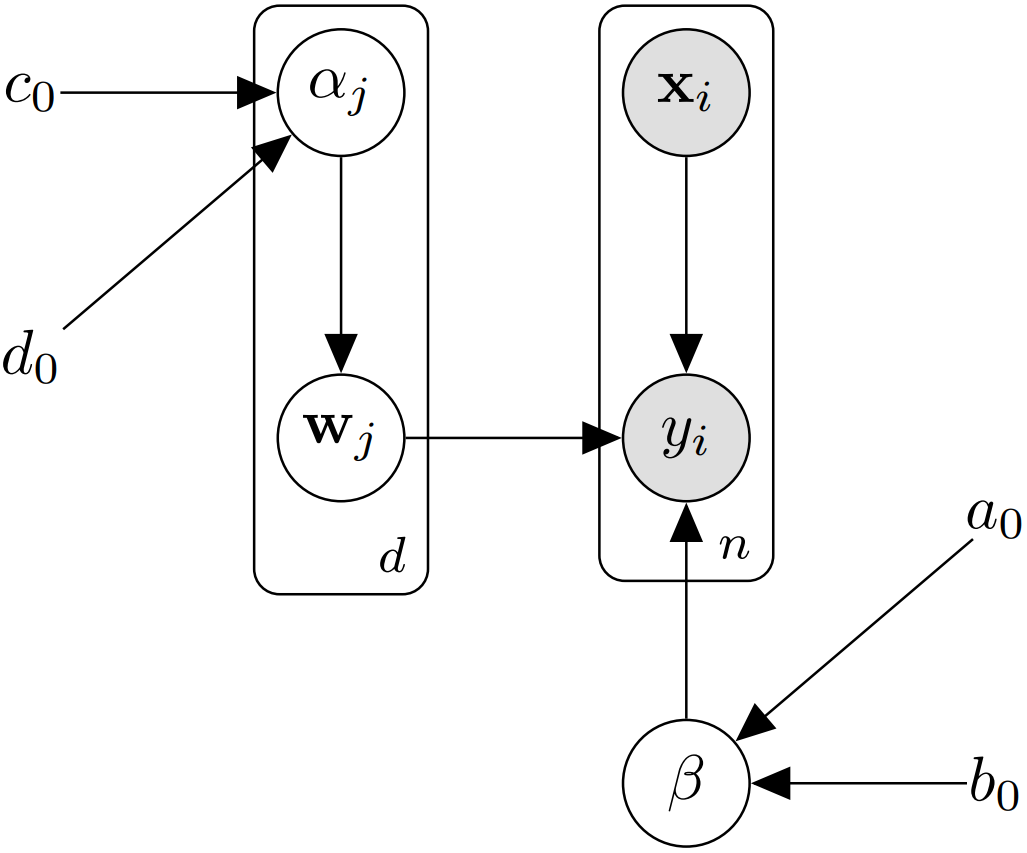
\includegraphics[scale=0.8]{bn_network.png}
	\caption{Plate diagram of the regression model with ARD prior. Variables $x_i$ , and $y_i$ are observed; We are interested in the posterior distribution of parameters $w$, $\alpha$ and $\beta$. The constants $a_0$ , $b_0$, $c_0$ , and $d_0$ are user-defined hyperparameters}
\end{figure}
\fi

\newcommand{\opGamma}{\operatorname{Gamma}}

\section{Introduction}
    This exercise is about using Gibbs sampling to estimate the posterior even with missing data. 

\section{Gibbs sampler}
    \subsection{Deriving conjugate prior for \texorpdfstring{$\mu$}{}}
        We assume here that we have the missing values, so we simply need to derive the conjugate prior 
        of the likelihood of the "assumed complete data". 
        \begin{align*}
            \log P(\mu|x,z) &= \sumlim{1}{n} \enclb{-\frac{1}{2}(x_i-\mu)^T \Sigma^{-1} (x_i-\mu)} \\ 
            &=-\frac{1}{2}\sumlim{1}{n} (x_i-\mu)^T \Sigma^{-1} (x_i-\mu) \\
            &=-\frac{1}{2}\sumlim{1}{n} x_i^T\Sigma^{-1}x_i - x_i^T\Sigma^{-1}\mu - \mu^T\Sigma^{-1}x_i +   \mu^T\Sigma^{-1}\mu\\
            &\propto -\frac{1}{2}\sumlim{1}{n} - 2x_i^T\Sigma^{-1}\mu + \mu^T\Sigma^{-1}\mu\\
            &= \sumlim{1}{n} x_i^T\Sigma^{-1}\mu - \frac{1}{2}\mu^T\Sigma^{-1}\mu\\
            &=  N\bar{X}^T\Sigma^{-1}\mu - \frac{1}{2}\mu^TN\Sigma^{-1}\mu\\
            &=  - \frac{1}{2}\mu^T\undertext{\Sigma^{-1}}{$=A$}\mu + \undertext{\bar{X}^T\Sigma^{-1}}{$=b^T$}\mu 
        \end{align*}
        Completing the square:
        \begin{align*}
            S &= A^{-1} = \Sigma \\ 
            m &= Sb = \Sigma \Sigma^{-1} \bar{X} = \bar{X}\\
            &\dunderline{\Rightarrow \mu \sim \mathcal{N}(\bar{X},\Sigma)} \\ 
            \text{For future self: }&\text{think before deriving something obvious!!!}
        \end{align*}
    
    \subsection{Deriving conjugate prior for \texorpdfstring{$Z$}{}}
        Conveniently, marginalizing away features from multivariate gaussians is simply done by dropping said features from the multivariate function \cite{marginalmvn}. In this case we will remain with a univariate Gaussian. Let $\sigma^2 = \Sigma_{11}$
        \begin{align*}
            P(Z|X,\mu) &= \prodlim[j]{1}{k} N(z_{j1}|\mu_1, \sigma)\\
            &\Rightarrow \dunderline{P(z_{j1}|\mu_1,\mu) = N(\mu_1,\Sigma_{11})}
        \end{align*}
    
    \subsection{Implementation}
    The implementation of the Gibbs sampler is then very simple. 
    \begin{enumerate}
        \item Initialize values for $Z$ and $\mu$
        \item For iterations $t$ in $T$ do:
        \begin{enumerate}[label*={\arabic*.}]
            \item Sample $\mu_t \sim \mathcal{N}(\bar{X}, \Sigma)$ ($X$ here is data with sampled $Z$ for missing data) 
            \item Sample $Z_t$ by sampling for each $z_{i1} \sim N(\mu_1, \Sigma_{11})$
        \end{enumerate}
    \end{enumerate}


\appendix

% \bibliographystyle{apalike}
\bibliographystyle{ieeetran}
\bibliography{citations}
    
\end{document}
    